\documentclass{beamer}
\mode<presentation>
\usepackage{amsmath,amssymb,mathtools}
\usepackage{textcomp}
\usepackage{gensymb}
\usepackage{adjustbox}
\usepackage{subcaption}
\usepackage{enumitem}
\usepackage{multicol}
\usepackage{listings}
\usepackage{url}
\usepackage{graphicx} % <-- needed for images
\def\UrlBreaks{\do\/\do-}

\usetheme{Boadilla}
\usecolortheme{lily}
\setbeamertemplate{footline}{
  \leavevmode%
  \hbox{%
  \begin{beamercolorbox}[wd=\paperwidth,ht=2ex,dp=1ex,right]{author in head/foot}%
    \insertframenumber{} / \inserttotalframenumber\hspace*{2ex}
  \end{beamercolorbox}}%
  \vskip0pt%
}
\setbeamertemplate{navigation symbols}{}

\lstset{
  frame=single,
  breaklines=true,
  columns=fullflexible,
  basicstyle=\ttfamily\tiny   % tiny font so code fits
}

\numberwithin{equation}{section}

% ---- your macros ----
\providecommand{\nCr}[2]{\,^{#1}C_{#2}}
\providecommand{\nPr}[2]{\,^{#1}P_{#2}}
\providecommand{\mbf}{\mathbf}
\providecommand{\pr}[1]{\ensuremath{\Pr\left(#1\right)}}
\providecommand{\qfunc}[1]{\ensuremath{Q\left(#1\right)}}
\providecommand{\sbrak}[1]{\ensuremath{{}\left[#1\right]}}
\providecommand{\lsbrak}[1]{\ensuremath{{}\left[#1\right.}}
\providecommand{\rsbrak}[1]{\ensuremath{\left.#1\right]}}
\providecommand{\brak}[1]{\ensuremath{\left(#1\right)}}
\providecommand{\lbrak}[1]{\ensuremath{\left(#1\right.}}
\providecommand{\rbrak}[1]{\ensuremath{\left.#1\right)}}
\providecommand{\cbrak}[1]{\ensuremath{\left\{#1\right\}}}
\providecommand{\lcbrak}[1]{\ensuremath{\left\{#1\right.}}
\providecommand{\rcbrak}[1]{\ensuremath{\left.#1\right\}}}
\theoremstyle{remark}
\newtheorem{rem}{Remark}
\newcommand{\sgn}{\mathop{\mathrm{sgn}}}
\providecommand{\abs}[1]{\left\vert#1\right\vert}
\providecommand{\res}[1]{\Res\displaylimits_{#1}}
\providecommand{\norm}[1]{\lVert#1\rVert}
\providecommand{\mtx}[1]{\mathbf{#1}}
\providecommand{\mean}[1]{E\left[ #1 \right]}
\providecommand{\fourier}{\overset{\mathcal{F}}{ \rightleftharpoons}}
\providecommand{\system}{\overset{\mathcal{H}}{ \longleftrightarrow}}
\providecommand{\dec}[2]{\ensuremath{\overset{#1}{\underset{#2}{\gtrless}}}}
\newcommand{\myvec}[1]{\ensuremath{\begin{pmatrix}#1\end{pmatrix}}}
\let\vec\mathbf

\title{MatGeo Presentation - Problem 2.5.32}
\author{EE25BTECH11064 - Yojit Manral}
\date{}

\begin{document}

\frame{\titlepage}
\begin{frame}{Question}
Show that the points $\brak{7,10}$, $\brak{-2,5}$ and $\brak{3,4}$ are vertices of an isosceles right triangle.
\end{frame}

\begin{frame}{Solution}
\begin{table}[h!]    
  \centering
  \begin{tabular}[12pt]{ |c| c|}
    \hline
    \textbf{Points} & \textbf{Name}\\ 
    \hline
	\myvec{7\\10} & Point $\Vec{A}$ \\
    \hline 
	\myvec{-2\\5} & Point $\Vec{B}$\\
    \hline
	\myvec{3\\4} & Point $\Vec{C}$\\
    \hline
\end{tabular}
  \caption{List of Points}
  \label{Table_1}
\end{table}

$\rightarrow$ The equation of the sides are given as
\begin{align}
    \vec{B}-\vec{A}=\myvec{-9\\-5} && \vec{C}-\vec{B}=\myvec{5\\-1} && \vec{A}-\vec{C}=\myvec{4\\6}
\end{align}
$\rightarrow$ The medians $\vec{D}$, $\vec{E}$ and $\vec{F}$ of the triangle are
\begin{align}
    \vec{D} = \frac{\vec{A}+\vec{B}}{2} = \myvec{5/2\\15/2} &&
    \vec{E} = \frac{\vec{B}+\vec{C}}{2} = \myvec{1/2\\9/2} &&
    \vec{F} = \frac{\vec{C}+\vec{A}}{2} = \myvec{5\\7}
\end{align}
\end{frame}

\begin{frame}{Solution}
\begin{enumerate}[label=(\Alph*)]
\item {
For an isosceles triangle, median to the base is also the perpendicular bisector. Using this property
\begin{align}
    (\vec{C}-\vec{D})^T(\vec{B}-\vec{A}) &= \myvec{1/2&-7/2}\myvec{-9\\-5} = 13 \neq 0 \\
    (\vec{A}-\vec{E})^T(\vec{C}-\vec{B}) &= \myvec{13/2&11/2}\myvec{5\\-1} = 27 \neq 0 \\
    (\vec{B}-\vec{F})^T(\vec{A}-\vec{C}) &= \myvec{-7&-2}\myvec{4\\6} = -40 \neq 0
\end{align}
$\rightarrow$ Since none of the sides satisfy this property, the triangle is not isosceles.
}
\end{enumerate}
\end{frame}

\begin{frame}{Solution}
\begin{enumerate}[label=(\Alph*)]\setcounter{enumi}{1}
\item {
For a right triangle, dot product of the perpendicular sides must be zero.
\begin{align}
    (\vec{B}-\vec{A})^T(\vec{C}-\vec{B})&=\myvec{-9&-5}\myvec{5\\-1} = -40 \neq 0 \\
    (\vec{C}-\vec{B})^T(\vec{A}-\vec{C})&=\myvec{5&-1}\myvec{4\\6} = 14 \neq 0 \\
    (\vec{A}-\vec{C})^T(\vec{B}-\vec{A})&=\myvec{4&6}\myvec{-9\\-5} = -66 \neq 0
\end{align}
$\rightarrow$ Since none of the dot products is zero, no two sides are perpendicular, and the triangle is not right angled.
}
\end{enumerate}
\end{frame}

\begin{frame}{Solution}
$\longrightarrow$ From (A) and (B), we get that $\triangle ABC$ is not isosceles right triangle.
\begin{figure}[h!]
   \centering
   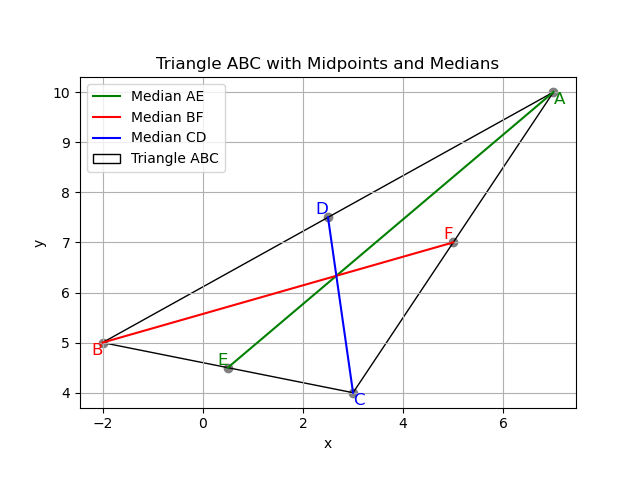
\includegraphics[width=0.75\linewidth]{figs/01.png}
   \caption{Plot of $\triangle$ABC}
   \label{Plot_1}
\end{figure}
\end{frame}

 % --------- CODE APPENDIX ---------
\section*{Appendix: Code}

% C program
\begin{frame}[fragile]{File: points.c}
\begin{lstlisting}[language=C]
#include <stdio.h>

int main() {
  FILE *fp;

  // -------------------
  // Question 2.5.32
  // -------------------


  fp = fopen("points.dat", "w");
  fprintf(fp, "%d,%d,%d\n", 7, 10, 0);  // A
  fprintf(fp, "%d,%d,%d\n", -2, 5, 0);   // B
  fprintf(fp, "%d,%d,%d\n", 3, 4, 0); // C
  fclose(fp);
  return 0;
  }
\end{lstlisting}
\end{frame}

% Python calling C
\begin{frame}[fragile]{File: call\_c.py}
\begin{lstlisting}[language=Python]
import subprocess

# Compile the C program
subprocess.run(["gcc", "points.c", "-o", "points"])

# Run the compiled C program
result = subprocess.run(["./points"], capture_output=True, text=True)

# Print the output from the C program
print(result.stdout)
\end{lstlisting}
\end{frame}

% Python plotting
\begin{frame}[fragile]{File: plot.py}
\begin{lstlisting}[language=Python]
import matplotlib.pyplot as plt

# Vertices of the triangle
A = (7, 10)
B = (-2, 5)
C = (3, 4)

# Midpoints of sides
D = ((A[0] + B[0]) / 2, (A[1] + B[1]) / 2)
E = ((B[0] + C[0]) / 2, (B[1] + C[1]) / 2)
F = ((A[0] + C[0]) / 2, (A[1] + C[1]) / 2)

# Plotting the triangle and midpoints
fig, ax = plt.subplots()

# Plot the triangle ABC
triangle = plt.Polygon([A, B, C], closed=True, fill=None, edgecolor='black', label='Triangle ABC')

# Plot the medians AD, BE, CF
plt.plot([A[0], E[0]], [A[1], E[1]], color='g', label='Median AE')
plt.plot([B[0], F[0]], [B[1], F[1]], color='r', label='Median BF')
plt.plot([C[0], D[0]], [C[1], D[1]], color='b', label='Median CD')
\end{lstlisting}
\end{frame}

\begin{frame}[fragile]{File: plot.py}
\begin{lstlisting}[language=Python]
# Plot the midpoints D, E, F
ax.scatter(*zip(A, B, C, D, E, F), color='gray')
ax.text(A[0], A[1], 'A', fontsize=12, ha='left', va='top', color='g')
ax.text(B[0], B[1], 'B', fontsize=12, ha='right', va='top', color='r')
ax.text(C[0], C[1], 'C', fontsize=12, ha='left', va='top', color='b')
ax.text(D[0], D[1], 'D', fontsize=12, ha='right', va='bottom', color='b')
ax.text(E[0], E[1], 'E', fontsize=12, ha='right', va='bottom', color='g')
ax.text(F[0], F[1], 'F', fontsize=12, ha='right', va='bottom', color='r')

# Labels and settings
ax.add_patch(triangle)
ax.set_aspect('equal', adjustable='box')
ax.set_xlabel('x')
ax.set_ylabel('y')
plt.title('Triangle ABC with Midpoints and Medians')
plt.grid(True)
plt.legend()
plt.show()
\end{lstlisting}
\end{frame}

\end{document}
